% =====================================================================
%  Product Requirements Document (PRD) - Mangan Yuk!
%  Kelompok 6 - II4011 Transformasi Digital
%
%  Kompilasi:  pdflatex main.tex  (jalankan 2x agar daftar isi terisi)
%              atau latexmk -pdf main.tex
% =====================================================================
\documentclass[11pt,letterpaper,oneside]{report}

% ---------- Bahasa & font ----------
\usepackage[T1]{fontenc}
\usepackage[utf8]{inputenc}
\usepackage[indonesian]{babel}
\usepackage{lmodern}
\usepackage{amssymb}
\usepackage{textcomp}

% ---------- Tata letak ----------
\usepackage[letterpaper,margin=2.5cm]{geometry}
\IfFileExists{pdflscape.sty}{\usepackage{pdflscape}}{\usepackage{lscape}}
\usepackage{setspace}
\setstretch{1.15}
\setlength{\parindent}{0pt}
\setlength{\parskip}{6pt}

% ---------- Tabel ----------
\usepackage{array}
\usepackage{longtable}
% Warna sel tabel butuh colortbl; jika tidak terpasang, warna dilewati.
\IfFileExists{colortbl.sty}{\usepackage[table]{xcolor}}{%
  \usepackage{xcolor}\newcommand{\cellcolor}[2][]{}\newcommand{\rowcolor}[2][]{}}
\usepackage{enumitem}
\newcolumntype{L}[1]{>{\raggedright\arraybackslash}p{\dimexpr#1\linewidth-2\tabcolsep-1.5\arrayrulewidth\relax}}
\renewcommand{\arraystretch}{1.25}
\setlist{nosep}
\setlist[itemize]{leftmargin=1.2em}
\AtBeginEnvironment{longtable}{\small}

% ---------- Gambar ----------
\usepackage{graphicx}
\usepackage{float}
\graphicspath{{images/}}

% ---------- Judul bab, header & footer ----------
\usepackage{titlesec}
\titleformat{\chapter}[hang]{\Large\bfseries}{\thechapter.}{0.6em}{}
\titlespacing*{\chapter}{0pt}{0pt}{12pt}
\titleformat{\section}{\large\bfseries}{\thesection}{0.6em}{}
\titleformat{\subsection}{\normalsize\bfseries}{\thesubsection}{0.6em}{}

\usepackage{fancyhdr}
\pagestyle{fancy}
\fancyhf{}
\renewcommand{\headrulewidth}{0pt}
\fancyfoot[L]{\footnotesize\textit{Template PRD - Tugas Besar Transformasi Digital}}
\fancyfoot[R]{\footnotesize\thepage}
\fancypagestyle{plain}{\fancyhf{}\fancyfoot[L]{\footnotesize\textit{Template PRD - Tugas Besar Transformasi Digital}}\fancyfoot[R]{\footnotesize\thepage}}

% ---------- Caption & tautan ----------
\usepackage[font=small,labelfont=bf]{caption}
\usepackage[hidelinks]{hyperref}
\usepackage{etoolbox}

\hypersetup{
  pdftitle={PRD Mangan Yuk! - Kelompok 6},
  pdfsubject={II4011 Transformasi Digital},
}

\begin{document}

% ===================== Bagian awal =====================
\pagenumbering{roman}
% Halaman sampul
\begin{titlepage}
\centering
\setstretch{1.2}

{\Large\bfseries PRODUCT REQUIREMENTS DOCUMENT (PRD)\par}
\vspace{0.6cm}
{\large Aplikasi Eksplorasi Kuliner Berdasarkan Lokasi dan Preferensi Pengguna\par}
\vspace{0.8cm}
{\Huge\bfseries ManganYuk!\par}
\vspace{0.3cm}
{\large Tempat Kuliner Sudirman Street, Bandung\par}
\vspace{0.8cm}
Mata Kuliah: II4011 Transformasi Digital\par
Dosen Pengajar: Prof. Ir. Kridanto Surendro, M.Sc., Ph.D.\par

\vspace{1cm}

\includegraphics[width=4cm]{images/logo-itb.png}\par
\vspace{1cm}

\textbf{Disusun Oleh:}\par
[06 / Copyright PPL]\par
\vspace{0.3cm}
\renewcommand{\arraystretch}{1.3}
\begin{tabular}{|c|l|c|}
\hline
\rowcolor[HTML]{D9EAF7}\textbf{No.} & \textbf{Nama Anggota} & \textbf{NIM} \\ \hline
1 & Dita Maheswari             & 13523125 \\ \hline
2 & Samantha Laqueenna Ginting & 13523138 \\ \hline
3 & Anggita Najmi Layali       & 18223122 \\ \hline
4 & Theresia Ivana M. S        & 18223126 \\ \hline
5 & Raka Adhitya Nugraha       & 18223013 \\ \hline
\end{tabular}

\vfill
{\bfseries PROGRAM STUDI SISTEM DAN TEKNOLOGI INFORMASI\\
SEKOLAH TEKNIK ELEKTRO DAN INFORMATIKA\\
INSTITUT TEKNOLOGI BANDUNG\\
2026\par}
\end{titlepage}

% Daftar isi, daftar tabel, dan daftar gambar
\setcounter{tocdepth}{2}
\tableofcontents
\clearpage
\listoftables
\clearpage
\listoffigures


% ===================== Isi (per bab) =====================
\clearpage
\pagenumbering{arabic}
% Bab 1: Product Definition
\chapter{Product Definition}
\label{bab:product-definition}
\section{Problem Statement}

Pengunjung kawasan kuliner seperti Sudirman Street Food, Bandung, dapat menghadapi kesulitan dalam mengeksplorasi berbagai pilihan kuliner ketika memiliki keterbatasan waktu dan anggaran. Informasi mengenai lokasi tenant, menu, dan harga dapat tersebar di berbagai sumber, sehingga pengguna perlu mencari dan membandingkan informasi secara terpisah sebelum menentukan tempat yang ingin dikunjungi. Kondisi ini berpotensi membuat proses eksplorasi kuliner menjadi kurang efisien, terutama ketika pengguna ingin mengunjungi beberapa tenant dalam satu waktu.

Hal ini membuka peluang transformasi digital melalui aplikasi eksplorasi kuliner berbasis lokasi yang mengintegrasikan informasi \textit{tenant }dengan konteks posisi pengguna. Dengan memanfaatkan lokasi pengguna, filter berdasarkan preferensi, serta rekomendasi tenant dan rute kunjungan, aplikasi dapat membantu pengguna menemukan pilihan kuliner yang relevan dengan waktu dan anggaran mereka tanpa harus berpindah-pindah platform.

\section{Target User/Stakeholder}

\begin{longtable}{|L{0.273}|L{0.354}|L{0.373}|}
\caption{Target User/Stakeholder}\\
\hline
\cellcolor[HTML]{D9EAF7}\textbf{Target User} & \cellcolor[HTML]{D9EAF7}\textbf{Karakteristik} & \cellcolor[HTML]{D9EAF7}\textbf{Kebutuhan Utama} \\ \hline
\endfirsthead
\hline
\cellcolor[HTML]{D9EAF7}\textbf{Target User} & \cellcolor[HTML]{D9EAF7}\textbf{Karakteristik} & \cellcolor[HTML]{D9EAF7}\textbf{Kebutuhan Utama} \\ \hline
\endhead
Pengunjung kawasan kuliner (lokal dan non-lokal) & Individu atau kelompok yang mengunjungi Sudirman Street Food; memiliki preferensi makanan, anggaran, dan waktu kunjungan yang berbeda & Menemukan tenant kuliner yang sesuai dengan anggaran, preferensi, dan lokasi; membandingkan pilihan berdasarkan informasi yang tersedia \\ \hline
Pengunjung dengan waktu terbatas & Pengunjung yang ingin mengeksplorasi beberapa tenant dalam satu kunjungan dengan durasi tertentu & Menentukan prioritas kunjungan dan menemukan rute sesuai waktu yang ia punya. \\ \hline
\end{longtable}

\section{Proposed Product}

\textbf{Mangan Yuk!} adalah aplikasi \textit{location-based culinary \& local culture explorer} yang membantu pengunjung dan wisatawan kawasan kuliner Sudirman Street Food untuk menemukan, menjelajahi, serta memahami ragam kuliner lokal beserta cerita budayanya secara efisien melalui pemicu lokasi \textit{hybrid} (GPS), \textit{Smart Culinary Trail Planner} berbasis preferensi (waktu, \textit{budget}, dan rasa), narasi audio multimodal, serta panduan navigasi interaktif, sehingga pengguna dapat menikmati pengalaman jelajah kuliner yang terstruktur, hemat waktu, dan kaya akan nilai budaya lokal tanpa perlu membuka banyak platform secara bersamaan.

\section{Product Goals \& Non-Goals}

\begin{longtable}{|L{0.500}|L{0.500}|}
\caption{Product Goals \& Non-Goals}\\
\hline
\cellcolor[HTML]{D9EAF7}\textbf{Product Goals} & \cellcolor[HTML]{D9EAF7}\textbf{Non-Goals} \\ \hline
\endfirsthead
\hline
\cellcolor[HTML]{D9EAF7}\textbf{Product Goals} & \cellcolor[HTML]{D9EAF7}\textbf{Non-Goals} \\ \hline
\endhead
G01. Membantu pengunjung menemukan rekomendasi tempat kuliner dan tenant berdasarkan lokasi/\textit{geofencing} saat eksplorasi di area studi kasus. & NG01. Versi awal tidak menyediakan sistem pemesanan makanan (\textit{online food ordering}) atau transaksi pembayaran digital (\textit{payment gateway}). \\ \hline
G02. Membantu pengguna membandingkan menu dan estimasi harga antar-tenant kuliner secara langsung dalam satu platform. & NG02. Versi awal tidak menggunakan fitur AI, kecerdasan buatan, maupun LLM (\textit{Large Language Model}) untuk sistem rekomendasi atau chatbot. \\ \hline
G03. Menyediakan peta interaktif dan navigasi rute untuk memandu pengguna menuju titik/tenant kuliner yang dituju. & NG03. Aplikasi tidak menyediakan pembaruan stok menu atau antrean secara \textit{real-time} dari pihak tenant (estimasi waktu kunjungan memakai rata-rata durasi hasil observasi). \\ \hline
G04. Membantu pengguna mengoptimalkan waktu kunjungan dengan memberikan estimasi waktu kunjungan dan pengingat durasi (\textit{dwelling time}). & NG04. Versi awal tidak mencakup seluruh area kuliner di Kota Bandung, melainkan berfokus khusus pada \textit{pilot project} di Sudirman Street Food. \\ \hline
G05. Mengirimkan notifikasi berbasis \textit{geofencing }(\textit{push notification}) saat pengguna memasuki radius atau lokasi area kuliner. & NG05. Aplikasi tidak menyediakan reservasi tempat duduk atau meja secara langsung untuk pengunjung. \\ \hline
\end{longtable}

% Bab 2: User Experience Scenario
\chapter{User Experience Scenario}
\label{bab:user-experience-scenario}
\section{Main Exploration Scenario}

\begin{longtable}{|L{0.500}|L{0.500}|}
\caption{Main Exploration Scenario}\\
\hline
\cellcolor[HTML]{D9EAF7}\textbf{{Aksi Aktor}} & \cellcolor[HTML]{D9EAF7}\textbf{{Reaksi Sistem}} \\ \hline
\endfirsthead
\hline
\cellcolor[HTML]{D9EAF7}\textbf{{Aksi Aktor}} & \cellcolor[HTML]{D9EAF7}\textbf{{Reaksi Sistem}} \\ \hline
\endhead
\multicolumn{2}{|L{1.000}|}{\textbf{Skenario Normal: Pengguna pertama kali memakai aplikasi, menjalankan Culinary Trail, lalu mencari tenant tambahan}} \\ \hline
Membuka aplikasi Mangan Yuk! untuk pertama kali &  \\ \hline
 & Menampilkan halaman login dengan tautan ke halaman registrasi \\ \hline
Mendaftar dengan nama pengguna, email, dan kata sandi &  \\ \hline
 & Menampilkan halaman onboarding (pengenalan aplikasi: jelajah kuliner, cerita budaya, culinary trail) \\ \hline
Menekan tombol Lanjut &  \\ \hline
 & Menampilkan penjelasan penggunaan lokasi (alasan, kapan lokasi dibaca, riwayat lokasi tidak dikirim ke server aplikasi, koordinat hanya dipakai layanan rute saat navigasi) dan tombol ``Izinkan Lokasi'' \\ \hline
Menekan tombol Izinkan Lokasi, lalu memilih ``Izinkan'' pada dialog sistem &  \\ \hline
 & Meminta izin notifikasi \\ \hline
Mengizinkan notifikasi &  \\ \hline
 & Meminta preferensi rasa (pedas/manis/gurih) dan jenis kuliner (makanan/minuman/jajanan), dengan opsi Lewati \\ \hline
Memilih preferensi pedas dan gurih, lalu menekan tombol Mulai &  \\ \hline
 & Menyimpan preferensi secara lokal, menampilkan Beranda (peta OSM + denah kawasan, posisi pengguna, status ``Di luar area'', jarak ke Sudirman Street Food, tombol Buka di Google Maps, Rencanakan Trail, dan Mode Jelajah) \\ \hline
Menekan tombol Buka di Google Maps &  \\ \hline
 & Membuka Google Maps dengan tujuan koordinat kawasan Sudirman Street Food \\ \hline
Menuju kawasan, kembali ke aplikasi, lalu mengaktifkan Mode Jelajah &  \\ \hline
 & Mengaktifkan pelacakan lokasi di background dan menampilkan notifikasi permanen ``Mangan Yuk! sedang memandu'' \\ \hline
Memasuki radius 100 m kawasan &  \\ \hline
 & Entry event: menampilkan notifikasi dan audio sambutan (``Selamat datang di Sudirman Street Food!''), menawarkan pilihan Rencanakan Trail atau Jelajah Bebas \\ \hline
Menekan notifikasi, lalu memilih Rencanakan Trail &  \\ \hline
 & Menampilkan form trail: durasi, budget, dan preferensi rasa (terisi otomatis dari onboarding) \\ \hline
Memilih durasi 60 menit, budget Rp50.000, lalu menekan tombol Buat Trail &  \\ \hline
 & Menampilkan itinerary 3 tenant berurutan beserta estimasi total biaya, estimasi waktu, dan rute di peta \\ \hline
Menekan tombol Mulai Trail &  \\ \hline
 & Menetapkan tenant pertama sebagai tujuan dan masuk mode navigasi (rute jalan kaki ke tujuan, jarak dalam meter, panah kompas), disertai audio ``Tenant pertama, 60 meter di depan'' \\ \hline
Memasukkan HP ke saku dan berjalan mengikuti arahan audio &  \\ \hline
 & Memberi panduan audio setiap jarak berkurang 20 m \\ \hline
Memasuki radius 25 m tenant pertama &  \\ \hline
 & Proximity event: HP bergetar dan memutar prompt ``Kamu mendekati [nama tenant]. Mau dengar ceritanya?'', notifikasi menampilkan tombol Dengar / Lewati \\ \hline
Menekan tombol Dengar dari lock screen &  \\ \hline
 & Memutar audio narasi cerita kuliner (asal-usul makanan, istilah Sunda, keunikan tenant) \\ \hline
Tiba dalam jarak \(\le\)10 m dari tenant &  \\ \hline
 & Memutar pengumuman ``Kamu sudah sampai!'' dan membuka kartu POI lengkap (foto, menu dan harga, cerita budaya, transkrip audio) \\ \hline
Memesan dan berada di tenant selama \(\ge\)3 menit &  \\ \hline
 & Dwell event: mencatat kunjungan secara otomatis dan menandai tenant pertama selesai pada trail \\ \hline
Masih makan di tenant melebihi alokasi waktu &  \\ \hline
 & Dwell event: mengirim notifikasi ``Sisa waktumu 30 menit, masih ada 2 tenant'' \\ \hline
Selesai makan dan berjalan keluar dari area tenant &  \\ \hline
 & Exit event: menampilkan tenant berikutnya beserta alasannya (misalnya ``30 m dari sini \(\cdot\) cocok setelah makanan pedas''), lalu masuk mode navigasi \\ \hline
Mengulangi alur navigasi, trigger, dan kunjungan untuk tenant kedua dan ketiga &  \\ \hline
 & Menjalankan trigger, memutar narasi, dan mencatat kunjungan otomatis untuk setiap tenant \\ \hline
Kunjungan di tenant terakhir selesai (dwell tercatat) &  \\ \hline
 & Menampilkan ringkasan trail (jumlah tenant, estimasi total belanja, durasi, dan jarak berjalan) \\ \hline
Menekan kolom pencarian dan mengetik ``batagr'' &  \\ \hline
 & Menampilkan hasil tenant batagor (toleran typo), diurutkan berdasarkan jarak \\ \hline
Memilih filter harga \textless{}Rp15rb, lalu memilih salah satu tenant &  \\ \hline
 & Menampilkan detail tenant dan tombol Jadikan Tujuan \\ \hline
Menekan tombol Jadikan Tujuan &  \\ \hline
 & Masuk mode navigasi menuju tenant yang dipilih \\ \hline
Tiba dalam jarak \(\le\)10 m dari tenant &  \\ \hline
 & Memutar pengumuman ``Kamu sudah sampai!'', membuka kartu POI, lalu mencatat kunjungan setelah pengguna berada \(\ge\)3 menit \\ \hline
Menekan tombol Selesai Jelajah &  \\ \hline
 & Mematikan pelacakan background, menghapus notifikasi permanen, dan kembali ke Beranda \\ \hline
\multicolumn{2}{|L{1.000}|}{\textbf{Skenario Alternatif 1: Pengguna menolak izin lokasi}} \\ \hline
Menekan ``Tolak'' pada dialog izin lokasi &  \\ \hline
 & Menampilkan penjelasan bahwa trigger otomatis dan navigasi tidak tersedia, dengan tombol Buka Pengaturan dan Lanjut tanpa Lokasi \\ \hline
Menekan tombol Lanjut tanpa Lokasi &  \\ \hline
 & Menampilkan peta tanpa posisi pengguna dan daftar tenant \\ \hline
Mengetuk salah satu tenant pada peta atau daftar &  \\ \hline
 & Menampilkan kartu POI dan tombol putar audio narasi (tanpa trigger otomatis dan navigasi) \\ \hline
\multicolumn{2}{|L{1.000}|}{\textbf{Skenario Alternatif 2: Pengguna memilih Jelajah Bebas}} \\ \hline
Memilih Jelajah Bebas pada notifikasi entry event &  \\ \hline
 & Menampilkan peta dengan seluruh marker tenant tanpa tujuan tertentu \\ \hline
Berkeliling kawasan tanpa tujuan &  \\ \hline
 & Memicu proximity event setiap kali pengguna mendekati tenant \\ \hline
Berhenti di tenant yang menarik \(\ge\)3 menit, lalu berjalan pergi &  \\ \hline
 & Mencatat kunjungan (dwell event), lalu saat exit event menampilkan 3 rekomendasi tenant berikutnya beserta alasannya \\ \hline
\multicolumn{2}{|L{1.000}|}{\textbf{Skenario Alternatif 3: Sinyal GPS lemah}} \\ \hline
Berjalan di area dengan sinyal GPS lemah (akurasi \textgreater{}30 m) &  \\ \hline
 & Mengabaikan pembacaan lokasi tersebut agar tidak terjadi trigger palsu, dan menampilkan banner ``Sinyal GPS lemah, trigger otomatis ditunda'' \\ \hline
Mengetuk daftar ``Tenant di sekitar'' atau marker tenant di peta &  \\ \hline
 & Menampilkan kartu POI dan audio narasi secara manual, lalu melanjutkan trigger otomatis setelah akurasi GPS kembali \(\le\)30 m \\ \hline
\multicolumn{2}{|L{1.000}|}{\textbf{Skenario Alternatif 4: Tenant pada trail tutup atau ingin dilewati}} \\ \hline
Menekan tombol Lewati Tenant pada mode navigasi &  \\ \hline
 & Menyusun ulang trail dengan tenant pengganti yang sedang buka, sesuai sisa waktu dan sisa budget, lalu menampilkan rute baru \\ \hline
\multicolumn{2}{|L{1.000}|}{\textbf{Skenario Alternatif 5: Pengguna menolak cerita saat proximity event}} \\ \hline
Menekan tombol Lewati pada notifikasi trigger &  \\ \hline
 & Menutup prompt audio, menyimpan tenant ke daftar ``Terlewati'', dan tidak memicu ulang tenant tersebut selama cooldown 30 menit \\ \hline
\multicolumn{2}{|L{1.000}|}{\textbf{Skenario Alternatif 6 (Optional): Pengguna mengumpulkan stempel Paspor Kuliner}} \\ \hline
Membuka menu Paspor Kuliner di Beranda &  \\ \hline
 & Menampilkan daftar trail tematik (misalnya ``Jejak Jajanan Sunda'' dan ``Manis-manis Bandung'') beserta progres masing-masing (misalnya 0/5) \\ \hline
Memilih trail ``Jejak Jajanan Sunda'' &  \\ \hline
 & Menampilkan daftar tenant yang termasuk trail tersebut dan menandainya di peta \\ \hline
Mengunjungi salah satu tenant pada trail dan berada di sana \(\ge\)3 menit &  \\ \hline
 & Dwell event: mencatat stempel digital untuk tenant tersebut, memutar efek suara singkat, dan memperbarui progres (1/5) \\ \hline
Mengunjungi tenant yang sama untuk kedua kalinya &  \\ \hline
 & Tidak mencatat stempel ganda; progres tetap 1/5 \\ \hline
Menutup aplikasi, lalu membukanya kembali di hari lain &  \\ \hline
 & Menampilkan progres paspor yang tersimpan (1/5) \\ \hline
Mengunjungi seluruh tenant pada trail hingga dwell tenant terakhir tercatat &  \\ \hline
 & Menampilkan badge ``Jejak Jajanan Sunda'' beserta audio ucapan selamat, dan menyimpan badge ke halaman Paspor Kuliner \\ \hline
\end{longtable}

\section{Main User Flow}

\begin{figure}[H]
\centering
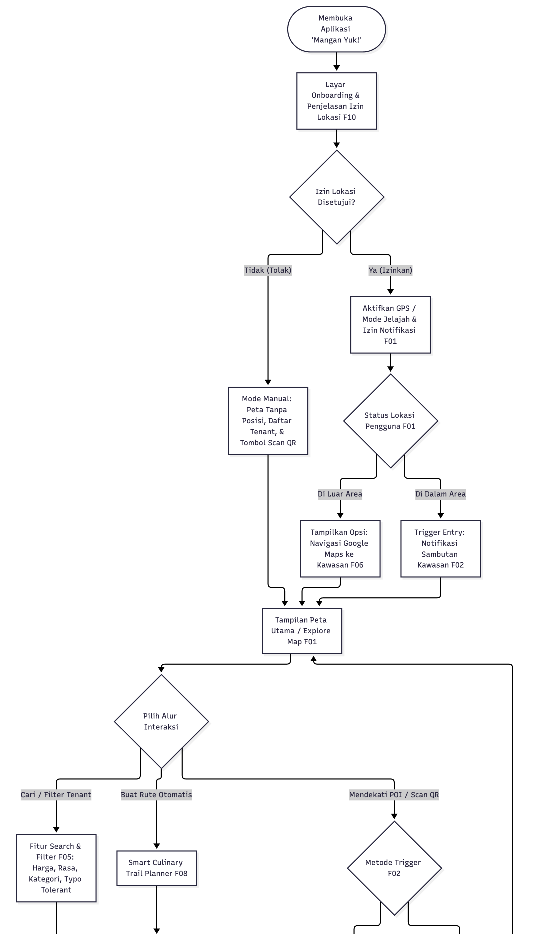
\includegraphics[width=0.9\textwidth,height=0.85\textheight,keepaspectratio]{images/user-flow-1.png}
\caption{Main User Flow aplikasi Mangan Yuk! (bagian 1 dari 3)}
\label{fig:user-flow-1}
\end{figure}

\begin{figure}[H]
\centering
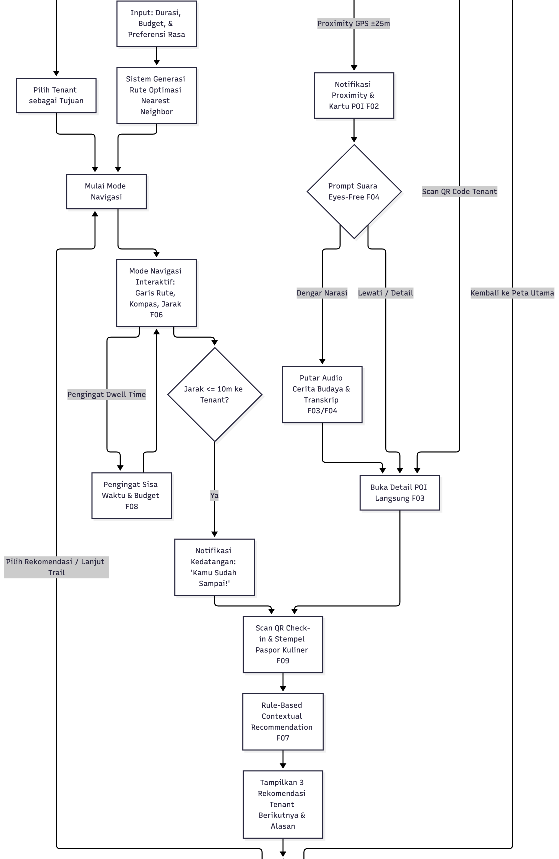
\includegraphics[width=0.9\textwidth,height=0.85\textheight,keepaspectratio]{images/user-flow-2.png}
\caption{Main User Flow aplikasi Mangan Yuk! (bagian 2 dari 3)}
\label{fig:user-flow-2}
\end{figure}

\begin{figure}[H]
\centering
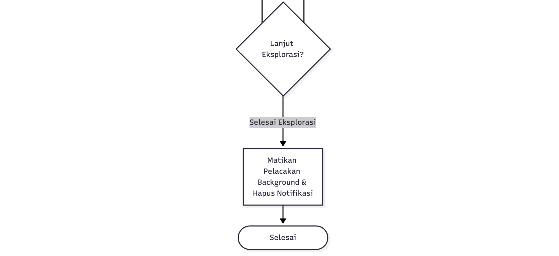
\includegraphics[width=0.9\textwidth,height=0.85\textheight,keepaspectratio]{images/user-flow-3.png}
\caption{Main User Flow aplikasi Mangan Yuk! (bagian 3 dari 3)}
\label{fig:user-flow-3}
\end{figure}

% Bab 3: Product Requirements - Baseline
\chapter{Product Requirements - Baseline}
\label{bab:product-requirements-baseline}
\begin{longtable}{|L{0.075}|L{0.226}|L{0.299}|L{0.093}|L{0.307}|}
\caption{Product Requirements - Baseline}\\
\hline
\cellcolor[HTML]{D9EAF7}\textbf{ID} & \cellcolor[HTML]{D9EAF7}\textbf{Requirement} & \cellcolor[HTML]{D9EAF7}\textbf{Deskripsi Implementasi} & \cellcolor[HTML]{D9EAF7}\textbf{Priority} & \cellcolor[HTML]{D9EAF7}\textbf{Acceptance Criteria} \\ \hline
\endfirsthead
\hline
\cellcolor[HTML]{D9EAF7}\textbf{ID} & \cellcolor[HTML]{D9EAF7}\textbf{Requirement} & \cellcolor[HTML]{D9EAF7}\textbf{Deskripsi Implementasi} & \cellcolor[HTML]{D9EAF7}\textbf{Priority} & \cellcolor[HTML]{D9EAF7}\textbf{Acceptance Criteria} \\ \hline
\endhead
F01 & Location Awareness & Aplikasi membaca posisi pengguna (akurasi tinggi, pembaruan tiap \(\pm\)3 detik atau perpindahan \(\ge\)5 m). Posisi ditampilkan sebagai titik biru dengan lingkaran akurasi di peta, disertai status ``Di dalam / di luar area Sudirman Street Food''. Jika izin lokasi ditolak, aplikasi berjalan dalam mode tanpa lokasi: peta dan daftar tenant tetap dapat dibuka secara manual, tetapi trigger otomatis dan navigasi tidak aktif. & Must & (1) Posisi tampil di peta \(\le\)10 detik setelah aplikasi dibuka dengan GPS aktif.\newline (2) Posisi diperbarui saat pengguna berjalan \(\ge\)5 m.\newline (3) Status di dalam/di luar area berubah dengan benar saat pengguna melewati batas area.\newline (4) Jika izin ditolak, muncul layar penjelasan dan konten tenant tetap dapat dibuka manual dari peta atau daftar. \\ \hline
F02 & Location-Based Trigger (Geofence) & Trigger sepenuhnya berbasis geofence GPS dengan empat jenis event:\begin{itemize}\item Entry event: geofence kawasan radius 100 m memunculkan notifikasi sambutan.\item Proximity event: geofence tenant radius 10 m (nilai \texttt{triggerRadiusM} per POI pada dataset) memunculkan kartu POI dan tawaran audio. Dicek dari pembaruan lokasi background dengan perhitungan jarak (haversine).\item Dwell event: pengguna berada di dalam geofence tenant \(\ge\)3 menit, sehingga kunjungan tercatat otomatis; jika melebihi alokasi trail, muncul pengingat sisa waktu (F08).\item Exit event: pengguna keluar dari geofence tenant, lalu muncul rekomendasi berikutnya (F07).\end{itemize}Pencegahan trigger palsu/berulang: pembacaan lokasi dengan akurasi \textgreater{}30 m diabaikan, hysteresis (exit tercatat jika jarak \textgreater{} radius + 10 m), dan cooldown 30 menit per POI. Trigger berjalan di background melalui foreground service selama ``Mode Jelajah'' aktif. & Must & (1) Notifikasi entry muncul \(\le\)15 detik setelah pengguna masuk area, termasuk saat aplikasi di background atau layar terkunci.\newline (2) Kartu POI muncul \(\le\)10 detik saat pengguna masuk radius POI, berhasil minimal 8 dari 10 percobaan lapangan.\newline (3) Trigger tidak muncul berulang selama pengguna tetap di area POI.\newline (4) Kunjungan tercatat setelah pengguna berada \(\ge\)3 menit di geofence tenant; pengguna yang hanya lewat (\textless{}3 menit) tidak tercatat berkunjung.\newline (5) Pembacaan lokasi dengan akurasi \textgreater{}30 m tidak memicu trigger. \\ \hline
F03 & Multimodal Exploration & Dataset memuat 31 POI tenant di Sudirman Street Food. Setiap POI memiliki: foto tenant/makanan (jika tersedia), kategori dan profil rasa, daftar menu dan harga, jam buka, serta audio narasi 45--90 detik (TTS) yang dilengkapi transkrip. Cerita kuliner/budaya (asal-usul makanan, keunikan tenant) disampaikan melalui narasi audio dan transkripnya. Seluruh konten (data JSON, foto, dan audio) dibundel di dalam APK sehingga dapat diakses offline. & Must & (1) 31/31 POI memiliki menu/harga, jam buka, serta audio narasi beserta transkrip.\newline (2) Audio dapat diputar, dijeda, dan dilanjutkan tanpa koneksi internet.\newline (3) Transkrip audio tersedia untuk setiap narasi.\newline (4) Konten POI terbuka \(\le\)2 detik. \\ \hline
F04 & Eyes-Free Interaction & Saat trigger terjadi, aplikasi memutar prompt suara, misalnya ``Kamu mendekati Batagor X. Mau dengar ceritanya?'', disertai getar. Pengguna merespons lewat tombol aksi di notifikasi (Dengar / Lewati) tanpa membuka aplikasi. Mode Jalan memutar narasi secara otomatis. Navigasi memberi panduan audio (``Tenant tujuan 20 meter lagi di sebelah kanan'') dan pengumuman saat tiba di tujuan. & Must & (1) Pengguna dapat memutar narasi dari notifikasi lock screen tanpa membuka aplikasi.\newline (2) Dalam Mode Jalan, narasi mulai \(\le\)3 detik setelah trigger.\newline (3) Panduan audio navigasi berbunyi minimal setiap pengurangan jarak 20 m dan saat tiba.\newline (4) Dalam usability test, minimal 4 dari 5 penguji dapat menyelesaikan satu kunjungan POI (navigasi, trigger, dan narasi) tanpa melihat layar. \\ \hline
F05 & Search \& Destination & Pencarian berdasarkan nama tenant, nama menu, atau kategori, dengan pencarian toleran typo. Filter yang tersedia: rentang harga (\textless{}Rp15rb, Rp15--30rb, \textgreater{}Rp30rb), rasa (pedas/manis/gurih), jenis (makanan/minuman/jajanan), dan status buka. Hasil diurutkan berdasarkan jarak, dan pengguna dapat menetapkan tenant sebagai tujuan. & Must & (1) Hasil pencarian muncul \(\le\)1 detik secara offline.\newline (2) Kata kunci ``batagor'' dan typo ``batagr'' sama-sama menampilkan tenant batagor.\newline (3) Kombinasi filter menghasilkan daftar yang sesuai.\newline (4) Tenant dapat dipilih sebagai tujuan dan langsung masuk ke mode navigasi. \\ \hline
F06 & Navigation & Menuju kawasan: membuka Google Maps melalui intent dengan koordinat kawasan.\newline Di dalam kawasan: peta (MapLibre dengan tile OpenStreetMap) menampilkan rute jalan kaki dari posisi pengguna ke tenant tujuan. Rute dihitung oleh layanan OSRM publik (profil pejalan kaki) dan dihitung ulang jika pengguna keluar \textgreater{}25 m dari rute; jika layanan gagal atau tidak ada koneksi, aplikasi memakai garis lurus. Peta juga menampilkan jarak dalam meter, dan panah arah berbasis kompas. Kedatangan terdeteksi saat jarak \(\le\)10 m, lalu aplikasi memutar pengumuman ``Kamu sudah sampai!'' dan membuka kartu POI tenant tujuan. & Must & (1) Jarak ke tujuan diperbarui saat pengguna berjalan.\newline (2) Panah menunjuk arah tujuan dengan deviasi \(\le\)30\textdegree{}.\newline (3) Notifikasi kedatangan muncul saat pengguna berada \(\le\)10 m dari tenant, dan kartu POI tenant tersebut terbuka.\newline (4) Navigasi dapat dilakukan ke 31/31 POI.\newline (5) Tombol ``Buka di Google Maps'' berfungsi dari luar kawasan.\newline (6) Tanpa koneksi internet, navigasi tetap berjalan dengan garis lurus ke tujuan. \\ \hline
F07 & Contextual Recommendation & Rekomendasi berbasis aturan (rule-based scoring) dengan faktor: jarak, status buka, kecocokan preferensi rasa, sisa budget, jam ramai (data observasi), dan status sudah/belum dikunjungi (dari dwell event). Muncul saat pengguna keluar dari geofence tenant yang sudah dikunjungi (exit event) dalam bentuk ``3 pilihan berikutnya'', masing-masing disertai alasan (misalnya ``30 m dari sini \(\cdot\) sesuai budget \(\cdot\) biasanya tidak ramai jam segini''). Ada juga aturan pasangan rasa, misalnya setelah makanan pedas disarankan minuman segar. & Must & (1) Rekomendasi tidak pernah memuat tenant yang tutup atau sudah dikunjungi.\newline (2) Setiap rekomendasi menampilkan alasannya.\newline (3) Rekomendasi muncul \(\le\)1 detik setelah exit event.\newline (4) Input yang sama selalu menghasilkan rekomendasi yang sama (deterministik). \\ \hline
F08 & Domain-Specific Innovative Feature: Smart Culinary Trail Planner & Pengguna mengisi waktu (30/60/90 menit), budget, dan preferensi rasa. Aplikasi memilih kombinasi tenant yang sesuai, lalu menyusun urutan rute dengan algoritma nearest neighbor, lengkap dengan estimasi total biaya dan waktu (dari data harga dan rata-rata durasi kunjungan hasil observasi). Progres trail diperbarui otomatis dari dwell event. Selama trail berjalan, dwell event juga memberi pengingat jika pengguna melewati alokasi waktu di satu tenant, misalnya ``Sisa waktumu 25 menit, masih ada 2 tenant.'' & Must & (1) Untuk input 60 menit dan Rp50.000, aplikasi menghasilkan itinerary minimal 2 tenant dengan estimasi biaya \(\le\) budget dan waktu \(\le\) durasi.\newline (2) Urutan rute tidak bolak-balik (setiap langkah menuju tenant terdekat berikutnya).\newline (3) Tenant pada trail otomatis ditandai selesai setelah dwell event tercatat.\newline (4) Notifikasi sisa waktu muncul saat dwell melebihi alokasi + 5 menit.\newline (5) Pengguna dapat melewati tenant atau menyusun ulang trail. \\ \hline
F09 & Location Privacy \& Consent & Layar onboarding menjelaskan alasan aplikasi memakai lokasi, kapan lokasi dibaca (hanya saat Mode Jelajah aktif), dan bahwa riwayat lokasi tidak dikirim ke server aplikasi. Riwayat posisi, kunjungan, dan progres trail hanya disimpan di perangkat. Satu-satunya pengiriman koordinat adalah saat navigasi aktif (F06): titik asal dan tujuan dikirim ke layanan rute OSRM publik untuk menghitung rute jalan kaki, tanpa identitas pengguna. Pengguna dapat mematikan Mode Jelajah kapan saja. & Must & (1) Penjelasan tampil sebelum permintaan izin sistem dan menyebut pemakaian layanan rute saat navigasi.\newline (2) Pelacakan background berhenti saat Mode Jelajah dimatikan (notifikasi foreground hilang).\newline (3) Tidak ada request jaringan ke server aplikasi yang membawa data lokasi; request yang membawa koordinat hanya ke layanan rute OSRM saat navigasi aktif (diverifikasi lewat log). \\ \hline
\end{longtable}

\section{Additional Requirements (Optional)}

\begin{longtable}{|L{0.082}|L{0.224}|L{0.296}|L{0.093}|L{0.304}|}
\caption{Additional Requirements (Optional)}\\
\hline
\cellcolor[HTML]{D9EAF7}\textbf{ID} & \cellcolor[HTML]{D9EAF7}\textbf{Requirement} & \cellcolor[HTML]{D9EAF7}\textbf{Deskripsi} & \cellcolor[HTML]{D9EAF7}\textbf{Priority} & \cellcolor[HTML]{D9EAF7}\textbf{Acceptance Criteria} \\ \hline
\endfirsthead
\hline
\cellcolor[HTML]{D9EAF7}\textbf{ID} & \cellcolor[HTML]{D9EAF7}\textbf{Requirement} & \cellcolor[HTML]{D9EAF7}\textbf{Deskripsi} & \cellcolor[HTML]{D9EAF7}\textbf{Priority} & \cellcolor[HTML]{D9EAF7}\textbf{Acceptance Criteria} \\ \hline
\endhead
F10 & Paspor Kuliner (Gamification) & Setiap kunjungan yang tercatat lewat dwell event (\(\ge\)3 menit di geofence tenant) memberi stempel digital; tidak ada scan QR. Tersedia trail tematik, misalnya ``Jejak Jajanan Sunda'' dan ``Manis-manis Bandung''. Badge diberikan saat satu trail selesai. Data disimpan lokal (AsyncStorage). & Could & (1) Stempel tercatat setelah dwell event dan tidak terduplikasi pada tenant yang sama.\newline (2) Progres trail tampil (misalnya 3/5).\newline (3) Badge muncul saat trail selesai.\newline (4) Data tetap ada setelah aplikasi ditutup dan dibuka kembali. \\ \hline
F11 & Akun Pengguna Lokal & Pengguna masuk atau mendaftar (email, nama pengguna, kata sandi) sebelum onboarding. Sesi disimpan di perangkat melalui SecureStore dan tidak dikirim ke server. Tersedia opsi ``Ingat Saya'' dan halaman Profil untuk melihat data akun, mengubah preferensi, dan keluar. & Could & (1) Pengguna yang belum masuk diarahkan ke halaman login.\newline (2) Setelah masuk, pengguna lanjut ke onboarding (pertama kali) atau Beranda.\newline (3) Sesi tetap tersimpan setelah aplikasi dibuka ulang.\newline (4) Keluar akun menghapus sesi dari perangkat. \\ \hline
\end{longtable}

% Bab 4: Point of Interest (POI) & Location-Trigger Design
\chapter{Point of Interest (POI) \& Location-Trigger Design}
\label{bab:point-of-interest-poi-location-trigger-design}
\section{POI Definition}

Dataset POI disimpan di \texttt{frontend/src/data/pois.json} dan dibundel di dalam APK. Dataset memuat 31 tenant di kawasan Sudirman Street Food (pusat kawasan $-6.92089$, $107.60057$; geofence kawasan radius 100 m). Semua POI memakai radius trigger 10 m (change log v1.1). Selain proximity event, setiap POI juga memicu dwell event (\(\ge\)3 menit di dalam radius) dan exit event (jarak \textgreater{} radius + 10 m), seperti dijelaskan pada F02. ID P02 dan P24 tidak dipakai.

\begin{landscapepage}
\begin{longtable}{|L{0.06}|L{0.17}|L{0.14}|L{0.14}|L{0.21}|L{0.11}|L{0.17}|}
\caption{POI Definition}\\
\hline
\cellcolor[HTML]{D9EAF7}\textbf{POI ID} & \cellcolor[HTML]{D9EAF7}\textbf{Nama POI} & \cellcolor[HTML]{D9EAF7}\textbf{Kategori} & \cellcolor[HTML]{D9EAF7}\textbf{Lokasi / Koordinat} & \cellcolor[HTML]{D9EAF7}\textbf{Content} & \cellcolor[HTML]{D9EAF7}\textbf{Trigger Rule} & \cellcolor[HTML]{D9EAF7}\textbf{System Response} \\ \hline
\endfirsthead
\hline
\cellcolor[HTML]{D9EAF7}\textbf{POI ID} & \cellcolor[HTML]{D9EAF7}\textbf{Nama POI} & \cellcolor[HTML]{D9EAF7}\textbf{Kategori} & \cellcolor[HTML]{D9EAF7}\textbf{Lokasi / Koordinat} & \cellcolor[HTML]{D9EAF7}\textbf{Content} & \cellcolor[HTML]{D9EAF7}\textbf{Trigger Rule} & \cellcolor[HTML]{D9EAF7}\textbf{System Response} \\ \hline
\endhead
\textbf{P01} & Traditional Fried Food from West Borneo & Gorengan / Manis-Gurih & (-6.92133, 107.60065) & 2 foto, 9 menu \& harga, jam buka, audio narasi 56s + transkrip & Proximity: masuk radius 10 m & Kartu POI, getar, dan prompt audio (Dengar/Lewati) \\ \hline
\textbf{P03} & Swike Asli JTW & Swike / Gurih & (-6.92129, 107.60065) & 1 foto, 19 menu \& harga, jam buka, audio narasi 53s + transkrip & Proximity: masuk radius 10 m & Kartu POI, getar, dan prompt audio (Dengar/Lewati) \\ \hline
\textbf{P04} & Bebek Gober Bumbu Hitam & Bebek / Gurih-Pedas & (-6.92129, 107.60060) & 2 foto, 11 menu \& harga, jam buka, audio narasi 54s + transkrip & Proximity: masuk radius 10 m & Kartu POI, getar, dan prompt audio (Dengar/Lewati) \\ \hline
\textbf{P05} & Pigbull & Nasi Campur / Gurih-Manis & (-6.92130, 107.60059) & 2 foto, 17 menu \& harga, jam buka, audio narasi 60s + transkrip & Proximity: masuk radius 10 m & Kartu POI, getar, dan prompt audio (Dengar/Lewati) \\ \hline
\textbf{P06} & Awin Kwetiau Siantar & Kwetiau / Gurih & (-6.92104, 107.60054) & 2 foto, 14 menu \& harga, jam buka, audio narasi 55s + transkrip & Proximity: masuk radius 10 m & Kartu POI, getar, dan prompt audio (Dengar/Lewati) \\ \hline
\textbf{P07} & Sedap The Best Chinese Food & Chinese Food / Gurih & (-6.92093, 107.60053) & 1 foto, 23 menu \& harga, jam buka, audio narasi 63s + transkrip & Proximity: masuk radius 10 m & Kartu POI, getar, dan prompt audio (Dengar/Lewati) \\ \hline
\textbf{P08} & Gou Cheng Hiang & Bak Kut Teh / Gurih & (-6.92093, 107.60046) & 1 foto, 21 menu \& harga, jam buka, audio narasi 59s + transkrip & Proximity: masuk radius 10 m & Kartu POI, getar, dan prompt audio (Dengar/Lewati) \\ \hline
\textbf{P09} & Dapur Sotoku & Soto \& Sop / Gurih & (-6.92084, 107.60047) & 1 foto, 12 menu \& harga, jam buka, audio narasi 57s + transkrip & Proximity: masuk radius 10 m & Kartu POI, getar, dan prompt audio (Dengar/Lewati) \\ \hline
\textbf{P10} & Klypot & Claypot \& Puding / Manis-Gurih & (-6.92078, 107.60048) & 1 foto, 15 menu \& harga, jam buka, audio narasi 60s + transkrip & Proximity: masuk radius 10 m & Kartu POI, getar, dan prompt audio (Dengar/Lewati) \\ \hline
\textbf{P11} & Umai & Japanese Food / Gurih-Pedas & (-6.92067, 107.60058) & 1 foto, 9 menu \& harga, jam buka, audio narasi 62s + transkrip & Proximity: masuk radius 10 m & Kartu POI, getar, dan prompt audio (Dengar/Lewati) \\ \hline
\textbf{P12} & Hong Nam & Bak Kut Teh / Gurih-Pedas & (-6.92069, 107.60048) & 1 foto, 19 menu \& harga, jam buka, audio narasi 51s + transkrip & Proximity: masuk radius 10 m & Kartu POI, getar, dan prompt audio (Dengar/Lewati) \\ \hline
\textbf{P13} & Pandu Baso Goreng Tenggiri & Bakso Goreng / Gurih & (-6.92069, 107.60048) & 1 foto, 4 menu \& harga, jam buka, audio narasi 53s + transkrip & Proximity: masuk radius 10 m & Kartu POI, getar, dan prompt audio (Dengar/Lewati) \\ \hline
\textbf{P14} & Segulung Babi & Nasi \& Bakmie Babi / Gurih-Pedas & (-6.92069, 107.60048) & 1 foto, 37 menu \& harga, jam buka, audio narasi 58s + transkrip & Proximity: masuk radius 10 m & Kartu POI, getar, dan prompt audio (Dengar/Lewati) \\ \hline
\textbf{P15} & Bacuk Sultan Agung & Nasi Goreng Babi / Gurih & (-6.92063, 107.60058) & 1 foto, 30 menu \& harga, jam buka, audio narasi 54s + transkrip & Proximity: masuk radius 10 m & Kartu POI, getar, dan prompt audio (Dengar/Lewati) \\ \hline
\textbf{P16} & Hau’s Tea & Cakue \& Bakso / Gurih & (-6.92063, 107.60058) & 3 foto, 15 menu \& harga, jam buka, audio narasi 55s + transkrip & Proximity: masuk radius 10 m & Kartu POI, getar, dan prompt audio (Dengar/Lewati) \\ \hline
\textbf{P17} & Kuo Tie Kelenteng & Kuo Tie / Gurih & (-6.92063, 107.60058) & 1 foto, 3 menu \& harga, jam buka, audio narasi 56s + transkrip & Proximity: masuk radius 10 m & Kartu POI, getar, dan prompt audio (Dengar/Lewati) \\ \hline
\textbf{P18} & Nasi Goreng Babi Samcan Crispy & Nasi Goreng / Gurih & (-6.92068, 107.60063) & 2 foto, 20 menu \& harga, jam buka, audio narasi 53s + transkrip & Proximity: masuk radius 10 m & Kartu POI, getar, dan prompt audio (Dengar/Lewati) \\ \hline
\textbf{P19} & Jazz Coffee & Kopi / Aromatik-Manis & (-6.92079, 107.60063) & 2 foto, 21 menu \& harga, jam buka, audio narasi 59s + transkrip & Proximity: masuk radius 10 m & Kartu POI, getar, dan prompt audio (Dengar/Lewati) \\ \hline
\textbf{P20} & Nasi Campur Kencana99 & Nasi Campur / Gurih & (-6.92056, 107.60139) & 2 foto, 35 menu \& harga, jam buka, audio narasi 59s + transkrip & Proximity: masuk radius 10 m & Kartu POI, getar, dan prompt audio (Dengar/Lewati) \\ \hline
\textbf{P21} & Kuwali Kwetiaw Bakar \& Nasi Goreng Samcan & Kwetiau / Gurih & (-6.92077, 107.60065) & 2 foto, 39 menu \& harga, jam buka, audio narasi 62s + transkrip & Proximity: masuk radius 10 m & Kartu POI, getar, dan prompt audio (Dengar/Lewati) \\ \hline
\textbf{P22} & Susu Mbok Darmi & Susu / Manis & (-6.92069, 107.60067) & 1 foto, 15 menu \& harga, jam buka, audio narasi 56s + transkrip & Proximity: masuk radius 10 m & Kartu POI, getar, dan prompt audio (Dengar/Lewati) \\ \hline
\textbf{P23} & D’Cheers & Bir \& Koktail / Segar & (-6.92120, 107.60060) & 2 foto, 27 menu \& harga, jam buka, audio narasi 58s + transkrip & Proximity: masuk radius 10 m & Kartu POI, getar, dan prompt audio (Dengar/Lewati) \\ \hline
\textbf{P25} & Medan & Bakmie Medan / Gurih & (-6.92115, 107.60054) & 4 foto, 36 menu \& harga, jam buka, audio narasi 59s + transkrip & Proximity: masuk radius 10 m & Kartu POI, getar, dan prompt audio (Dengar/Lewati) \\ \hline
\textbf{P26} & Sotomie Sukabumi Ko Ricky \& Happy Time & Mie Berkuah / Gurih & (-6.92101, 107.60048) & 1 foto, 45 menu \& harga, jam buka, audio narasi 50s + transkrip & Proximity: masuk radius 10 m & Kartu POI, getar, dan prompt audio (Dengar/Lewati) \\ \hline
\textbf{P27} & Rainbow Juice & Jus / Segar-Manis & (-6.92075, 107.60055) & belum ada foto, 44 menu \& harga, jam buka, audio narasi 57s + transkrip & Proximity: masuk radius 10 m & Kartu POI, getar, dan prompt audio (Dengar/Lewati) \\ \hline
\textbf{P28} & Pempek Gochan & Pempek / Gurih & (-6.92071, 107.60061) & 1 foto, 32 menu \& harga, jam buka, audio narasi 58s + transkrip & Proximity: masuk radius 10 m & Kartu POI, getar, dan prompt audio (Dengar/Lewati) \\ \hline
\textbf{P29} & Mie Susu & Mie \& Ronde / Manis-Gurih & (-6.92066, 107.60065) & 2 foto, 7 menu \& harga, jam buka, audio narasi 56s + transkrip & Proximity: masuk radius 10 m & Kartu POI, getar, dan prompt audio (Dengar/Lewati) \\ \hline
\textbf{P30} & Waroenk Laris & Samcan / Gurih-Pedas & (-6.92071, 107.60062) & belum ada foto, 20 menu \& harga, jam buka, audio narasi 67s + transkrip & Proximity: masuk radius 10 m & Kartu POI, getar, dan prompt audio (Dengar/Lewati) \\ \hline
\textbf{P31} & Bacang Babi & Bacang \& Bakpao / Gurih-Manis & (-6.92066, 107.60066) & 1 foto, 13 menu \& harga, jam buka, audio narasi 57s + transkrip & Proximity: masuk radius 10 m & Kartu POI, getar, dan prompt audio (Dengar/Lewati) \\ \hline
\textbf{P32} & Sate Babi Wibisana & Sate / Gurih-Pedas & (-6.92120, 107.60062) & 3 foto, 21 menu \& harga, jam buka, audio narasi 60s + transkrip & Proximity: masuk radius 10 m & Kartu POI, getar, dan prompt audio (Dengar/Lewati) \\ \hline
\textbf{P33} & El Paso & Meksiko / Gurih & (-6.92086, 107.60057) & 2 foto, 14 menu \& harga, jam buka, audio narasi 56s + transkrip & Proximity: masuk radius 10 m & Kartu POI, getar, dan prompt audio (Dengar/Lewati) \\ \hline
\end{longtable}
\end{landscapepage}

\section{Location-Trigger Logic}

\subsection{Diagram Location-Trigger Logic}

\begin{figure}[H]
\centering
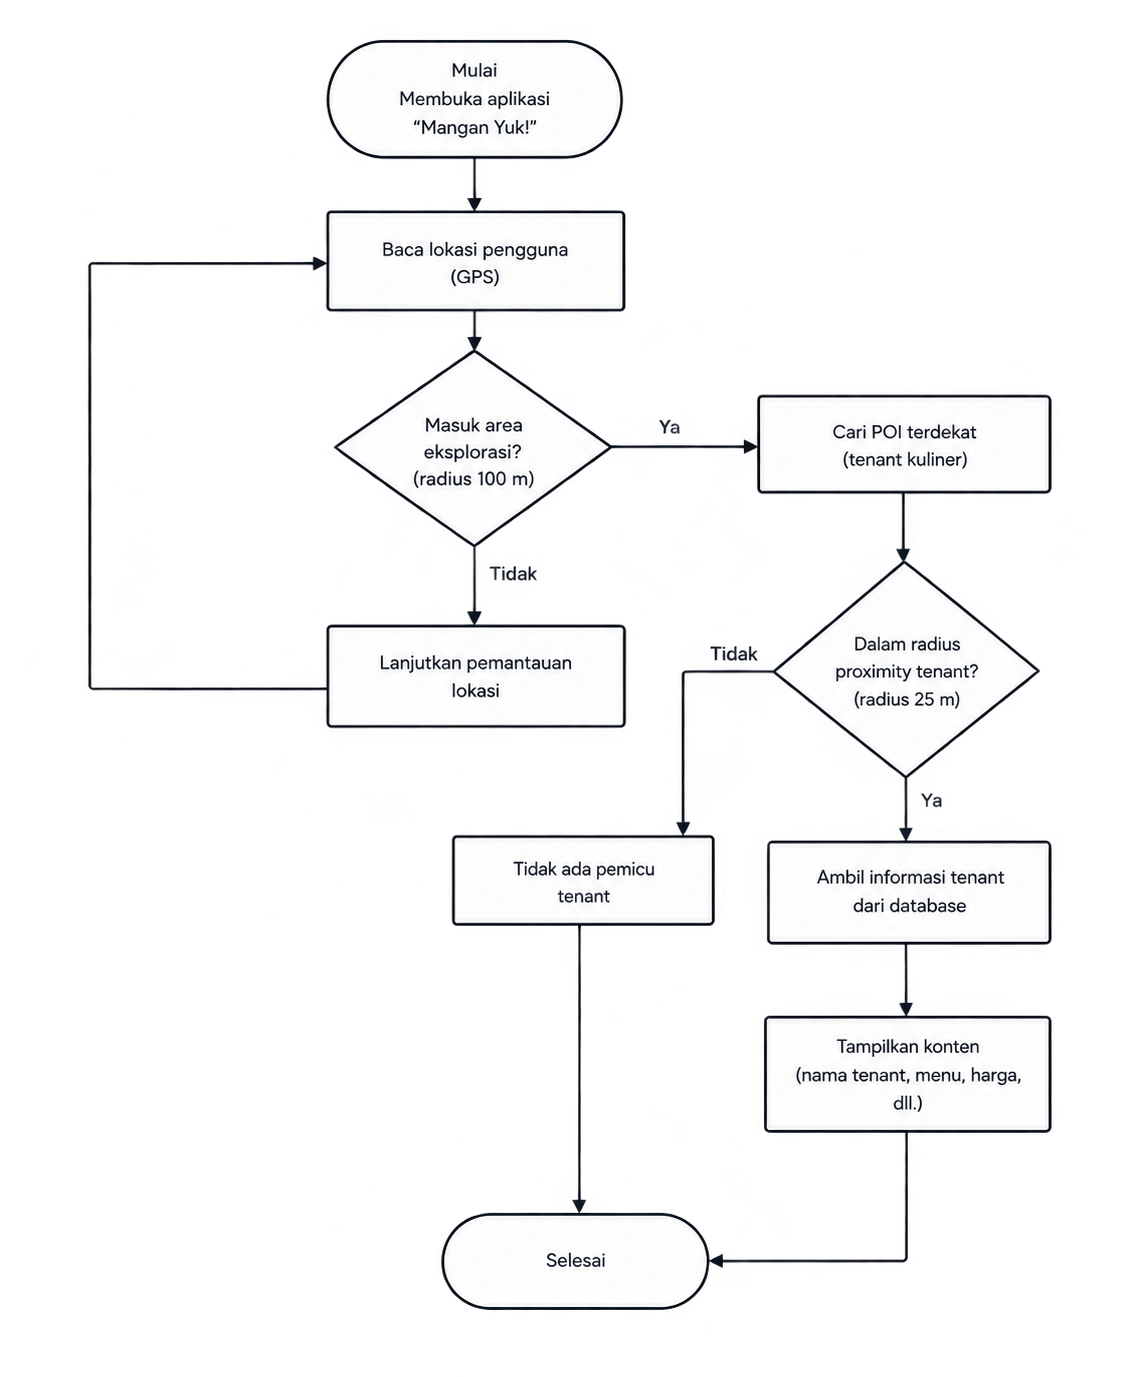
\includegraphics[width=0.6\textwidth,height=0.8\textheight,keepaspectratio]{images/diagram-location-trigger.png}
\caption{Diagram Location-Trigger Logic}
\label{fig:diagram-location-trigger}
\end{figure}

\subsection{Penjelasan Alur Logika}
\begin{enumerate}
  \item Pembacaan lokasi: aplikasi meminta izin lokasi kepada pengguna dan membaca koordinat GPS secara berkala ketika fitur eksplorasi aktif.
  \item Identifikasi POI: sistem mencari tenant yang berada dalam radius tertentu dari posisi pengguna.
  \item Pemeriksaan kondisi: sistem memeriksa apakah pengguna telah memasuki radius pemicu dan apakah informasi tenant tersebut sudah ditampilkan dalam sesi eksplorasi saat ini.
  \item Pemilihan konten: jika kondisi terpenuhi, sistem mengambil informasi tenant dari basis data. Informasi yang ditampilkan menggunakan data terstruktur dan aturan yang ditetapkan, bukan hasil generasi LLM.
  \item Respons sistem: aplikasi menampilkan kartu informasi atau pop-up. Pengguna dapat melihat detail tenant, membandingkan pilihan, atau melanjutkan ke POI berikutnya.
\end{enumerate}

\subsection{Contoh Skenario}

Radius pemicu setiap tenant adalah 10 meter. Ketika pengguna mendekati tenant tersebut hingga masuk ke radius itu, aplikasi memeriksa status pemicu. Jika informasinya belum ditampilkan pada sesi eksplorasi, aplikasi menampilkan kartu berisi nama tenant, kategori makanan, menu, dan harga. Jika pengguna masih berada di radius yang sama, \textit{pop-up} tidak ditampilkan berulang kali.

% Bab 5: Low-Fidelity Prototype
\chapter{Low-Fidelity Prototype}
\label{bab:low-fidelity-prototype}
\section{Screen/State List}

Daftar layar sesuai implementasi di \texttt{frontend/app}.

\begin{longtable}{|L{0.092}|L{0.184}|L{0.507}|L{0.217}|}
\caption{Screen/State List}\\
\hline
\cellcolor[HTML]{D9EAF7}\textbf{ID} & \cellcolor[HTML]{D9EAF7}\textbf{Screen/State} & \cellcolor[HTML]{D9EAF7}\textbf{Tujuan} & \cellcolor[HTML]{D9EAF7}\textbf{Related Requirement} \\ \hline
\endfirsthead
\hline
\cellcolor[HTML]{D9EAF7}\textbf{ID} & \cellcolor[HTML]{D9EAF7}\textbf{Screen/State} & \cellcolor[HTML]{D9EAF7}\textbf{Tujuan} & \cellcolor[HTML]{D9EAF7}\textbf{Related Requirement} \\ \hline
\endhead
UI01 & Login \& Registrasi (\texttt{auth/login}, \texttt{auth/register}) & Masuk atau membuat akun lokal sebelum memakai aplikasi & F11 \\ \hline
UI02 & Onboarding: Welcome & Memperkenalkan aplikasi: jelajah kuliner, cerita budaya, culinary trail & F09 \\ \hline
UI03 & Onboarding: Izin Lokasi & Menjelaskan pemakaian lokasi lalu meminta izin sistem & F01, F09 \\ \hline
UI04 & Onboarding: Tanpa Lokasi & Menjelaskan fitur yang tidak tersedia jika izin lokasi ditolak & F01, F09 \\ \hline
UI05 & Onboarding: Izin Notifikasi & Meminta izin notifikasi untuk trigger dan pengingat & F02, F04 \\ \hline
UI06 & Onboarding: Preferensi & Memilih preferensi rasa, jenis kuliner, dan opsi hanya tenant halal & F07, F08, F12 \\ \hline
UI07 & Explore (Beranda/Peta) & Menampilkan posisi pengguna, batas kawasan, marker POI, status area, jarak ke kawasan, dan Mode Jelajah & F01, F02, F06, F09 \\ \hline
UI08 & POI Trigger Notification & Notifikasi entry/proximity dengan tombol Dengar / Lewati di lock screen & F02, F04 \\ \hline
UI09 & POI Detail (\texttt{poi/[id]}) & Menampilkan foto, menu dan harga, jam buka, status halal, audio narasi, transkrip, serta ringkasan dan daftar ulasan & F03, F04, F10 \\ \hline
UI10 & Search & Pencarian toleran typo dengan filter harga, rasa, jenis, dan status buka & F05 \\ \hline
UI11 & Navigasi (\texttt{navigate/[poiId]}) & Rute jalan kaki, jarak, panah kompas, panduan audio, dan deteksi kedatangan & F04, F06 \\ \hline
UI12 & Trail Planner & Input durasi, budget, dan preferensi rasa untuk membuat trail & F08 \\ \hline
UI13 & Trail Itinerary & Urutan tenant, estimasi biaya dan waktu, progres, serta Lewati Tenant & F07, F08 \\ \hline
UI14 & Trail Summary & Ringkasan trail: jumlah tenant, total belanja, durasi, dan jarak & F08 \\ \hline
UI15 & Paspor Kuliner (\texttt{passport}) & Trail tematik, stempel digital, progres, badge, riwayat ulasan, dan tombol Tambah Ulasan & F10 \\ \hline
UI16 & Profil \& Pengaturan & Data akun, ringkasan paspor, edit preferensi (termasuk halal), akses paspor, halaman pengaturan, dan keluar akun & F09, F11, F12 \\ \hline
UI17 & Form Ulasan (modal) & Memilih tenant, memberi rating 1--5, memilih menu yang dimakan, menulis ulasan, dan mengunggah foto & F10 \\ \hline
\end{longtable}

\section{Wireframe}

\textit{Masukkan low-fidelity wireframe untuk screen/state utama. Prototype perlu memperlihatkan perubahan kondisi ketika pengguna masih berada di luar area POI, mulai mendekati POI, menerima pemicu, dan kemudian mengakses informasi eksplorasi.}

\textit{[Tempel low-fidelity prototype di sini]}

% Bab 6: Product Backlog
\chapter{Product Backlog}
\label{bab:product-backlog}
\begin{longtable}{|L{0.118}|L{0.281}|L{0.172}|L{0.107}|L{0.208}|L{0.114}|}
\caption{Product Backlog}\\
\hline
\cellcolor[HTML]{D9EAF7}\textbf{Backlog ID} & \cellcolor[HTML]{D9EAF7}\textbf{Product Backlog Item} & \cellcolor[HTML]{D9EAF7}\textbf{Related Req.} & \cellcolor[HTML]{D9EAF7}\textbf{Priority} & \cellcolor[HTML]{D9EAF7}\textbf{Acceptance / Done Criteria} & \cellcolor[HTML]{D9EAF7}\textbf{Target Sprint} \\ \hline
\endfirsthead
\hline
\cellcolor[HTML]{D9EAF7}\textbf{Backlog ID} & \cellcolor[HTML]{D9EAF7}\textbf{Product Backlog Item} & \cellcolor[HTML]{D9EAF7}\textbf{Related Req.} & \cellcolor[HTML]{D9EAF7}\textbf{Priority} & \cellcolor[HTML]{D9EAF7}\textbf{Acceptance / Done Criteria} & \cellcolor[HTML]{D9EAF7}\textbf{Target Sprint} \\ \hline
\endhead
PB01 & Menyiapkan project aplikasi dan struktur navigasi halaman yang dapat dijalankan pada perangkat uji & - & Must & Aplikasi berhasil dibuka tanpa crash dan perpindahan antarhalaman utama berjalan & S1 \\ \hline
PB02 & Mengimplementasikan onboarding, penjelasan privasi lokasi, serta permintaan izin lokasi dan notifikasi & F09, F01 & Must & Penjelasan tampil sebelum dialog izin sistem; jika izin ditolak, aplikasi masuk mode tanpa lokasi & S1 \\ \hline
PB03 & Mengimplementasikan pembacaan lokasi pengguna dan menampilkannya di peta beserta status di dalam/di luar area & F01 & Must & Posisi tampil \(\le\)10 detik, diperbarui saat berpindah \(\ge\)5 m, dan status area berubah dengan benar & S1 \\ \hline
PB04 & Menyusun dataset minimal 10 POI (koordinat, menu, harga, jam buka, rasa, kategori) & F01, F02, F03 & Must & Data 10 POI dapat dibaca aplikasi dan ditampilkan sebagai marker di peta & S1 \\ \hline
PB05 & Mengimplementasikan Mode Jelajah dengan pelacakan lokasi di background & F02, F09 & Must & Notifikasi permanen muncul saat Mode Jelajah aktif dan pelacakan berhenti saat dimatikan & S2 \\ \hline
PB06 & Mengimplementasikan geofence entry event dan proximity event, termasuk pencegahan trigger palsu & F02 & Must & Notifikasi entry \(\le\)15 detik; kartu POI \(\le\)10 detik; akurasi \textgreater{}30 m diabaikan; trigger tidak berulang (cooldown 30 menit) & S2 \\ \hline
PB07 & Mengimplementasikan dwell event dan exit event untuk pencatatan kunjungan otomatis & F02 & Must & Kunjungan tercatat setelah \(\ge\)3 menit di geofence; pengguna yang hanya lewat tidak tercatat; exit menggunakan hysteresis & S2 \\ \hline
PB08 & Membuat kartu POI multimodal (foto, deskripsi, cerita budaya, menu \& harga, audio narasi + transkrip) yang dapat diakses offline & F03 & Must & 10/10 POI memiliki konten lengkap, konten terbuka \(\le\)2 detik, dan audio dapat diputar/dijeda tanpa internet & S2 \\ \hline
PB09 & Mengimplementasikan interaksi eyes-free: prompt suara, getar, tombol Dengar/Lewati di notifikasi, dan Mode Jalan & F04 & Must & Narasi dapat diputar dari lock screen; dalam Mode Jalan, narasi mulai \(\le\)3 detik setelah trigger & S3 \\ \hline
PB10 & Mengimplementasikan pencarian toleran typo dan filter tenant (harga, rasa, jenis, status buka) & F05 & Must & Hasil muncul \(\le\)1 detik secara offline; ``batagr'' menampilkan tenant batagor; kombinasi filter sesuai & S3 \\ \hline
PB11 & Mengimplementasikan navigasi menuju kawasan (Google Maps) dan di dalam kawasan (garis rute, jarak, kompas, panduan audio) & F06, F04 & Must & Panah deviasi \(\le\)30\textdegree{}; panduan audio tiap 20 m; kedatangan \(\le\)10 m membuka kartu POI; navigasi berhasil ke 10/10 POI & S3 \\ \hline
PB12 & Mengintegrasikan alur eksplorasi utama (lokasi \(\rightarrow\) trigger \(\rightarrow\) kartu POI \(\rightarrow\) navigasi) untuk Major Progress Review & F01--F06 & Must & Satu skenario kunjungan POI dapat didemokan end-to-end di perangkat uji & S3 \\ \hline
PB13 & Mengimplementasikan rekomendasi kontekstual berbasis aturan (rule-based scoring) & F07 & Must & Muncul \(\le\)1 detik setelah exit event; menampilkan 3 tenant beserta alasan; tidak memuat tenant tutup/sudah dikunjungi; hasil deterministik & S4 \\ \hline
PB14 & Mengimplementasikan Smart Culinary Trail Planner (input durasi, budget, rasa \(\rightarrow\) itinerary nearest neighbor) & F08 & Must & Input 60 menit \& Rp50.000 menghasilkan \(\ge\)2 tenant dengan biaya \(\le\) budget, waktu \(\le\) durasi, dan rute tidak bolak-balik & S4 \\ \hline
PB15 & Mengimplementasikan progres trail, pengingat sisa waktu, serta fitur lewati tenant/susun ulang trail & F08, F02 & Must & Tenant ditandai selesai setelah dwell; notifikasi muncul saat dwell melebihi alokasi + 5 menit; trail dapat disusun ulang & S4 \\ \hline
PB16 & Mengimplementasikan Paspor Kuliner (stempel digital, trail tematik, badge) & F10 & Could & Stempel tidak terduplikasi; progres tampil (misalnya 3/5); badge muncul; data tetap ada setelah aplikasi dibuka ulang & S4 \\ \hline
PB17 & Melakukan pengujian acceptance criteria (uji lapangan, usability test, verifikasi log jaringan) & F01--F10 & Must & Trigger berhasil \(\ge\)8/10 percobaan; \(\ge\)4/5 penguji menyelesaikan kunjungan tanpa melihat layar; tidak ada request ke backend Mangan Yuk yang berisi koordinat pengguna, dan koordinat hanya dikirim ke OSRM selama navigasi aktif & S5 \\ \hline
PB18 & Memperbaiki defect, melakukan retest, dan menstabilkan build akhir & - & Must & Seluruh defect prioritas tinggi tertutup, retest lulus, dan build final berjalan tanpa crash & S5 \\ \hline
\end{longtable}

% Bab 7: Sprint Plan
% Sumber: docs/scrum-document.md (2.3 Release Planning dan Tabel Sprint Backlog 1-5)
\chapter{Sprint Plan}
\label{bab:sprint-plan}
\textit{Sprint berlangsung satu minggu. Sprint plan awal dapat disesuaikan selama proyek, tetapi perubahan backlog/requirement harus dapat ditelusuri.}

\newcommand{\sprinthead}{%
\cellcolor[HTML]{D9EAF7}\textbf{ID Task} & \cellcolor[HTML]{D9EAF7}\textbf{Rincian Task} & \cellcolor[HTML]{D9EAF7}\textbf{Est. (Jam)} & \cellcolor[HTML]{D9EAF7}\textbf{Backlog ID} & \cellcolor[HTML]{D9EAF7}\textbf{PIC} \\ \hline}
\newenvironment{sprinttable}[1]{%
\begin{longtable}{|L{0.11}|L{0.50}|L{0.09}|L{0.11}|L{0.19}|}
\caption{#1}\\
\hline
\sprinthead
\endfirsthead
\hline
\sprinthead
\endhead}{\end{longtable}}

\section*{Sprint 1 - Week 10}
\addcontentsline{toc}{section}{Sprint 1 - Week 10}

\textbf{Periode:} 23 Februari -- 1 Maret 2026\\
\textbf{Sprint Goal:} Membangun fondasi arsitektur aplikasi, menyelesaikan onboarding dan edukasi privasi lokasi, menampilkan posisi GPS pengguna di peta OSM secara real-time, serta membundel dataset POI Sudirman Street Food.\\
\textbf{Target Increment:} Aplikasi dapat dijalankan di perangkat uji, onboarding dan izin lokasi berjalan, posisi pengguna dan status di dalam/di luar area tampil di peta, dan marker POI terbaca dari dataset lokal.\\
\textbf{Backlog:} PB01, PB02, PB03, PB04 (estimasi 48 jam tim)

\begin{sprinttable}{Sprint Backlog 1 - Week 10}
SB-1.1 & Inisialisasi project React Native Expo (TypeScript), struktur folder modular, konfigurasi ESLint, Prettier, dan navigasi stack/tab. & 8 & PB01 & Samantha \\ \hline
SB-1.2 & Perancangan UI onboarding, dialog transparansi privasi lokasi (F09), dan penanganan penolakan izin lokasi. & 8 & PB02 & Anggita \\ \hline
SB-1.3 & Implementasi alur permintaan izin lokasi foreground dan notifikasi dengan fallback mode tanpa lokasi. & 6 & PB02 & Samantha \\ \hline
SB-1.4 & Integrasi peta (MapLibre) dengan tile OpenStreetMap dan poligon batas kawasan Sudirman Street Food. & 10 & PB03 & Samantha \\ \hline
SB-1.5 & Implementasi pembacaan GPS akurasi tinggi (\texttt{watchPositionAsync}), titik biru pengguna, dan kalkulasi status di dalam/di luar area. & 8 & PB03 & Dita \\ \hline
SB-1.6 & Survei, kurasi, dan penyusunan JSON dataset POI tenant kuliner (nama, koordinat, menu, harga, kategori, rasa). & 8 & PB04 & Theresia, Anggita \\ \hline
\end{sprinttable}

\section*{Sprint 2 - Week 11}
\addcontentsline{toc}{section}{Sprint 2 - Week 11}

\textbf{Periode:} 2 -- 8 Maret 2026\\
\textbf{Sprint Goal:} Mengimplementasikan pelacakan lokasi background (Mode Jelajah melalui foreground service), mesin geofence (entry, proximity, dwell, exit) dengan pencegahan trigger palsu, serta kartu POI multimodal offline dengan pemutar audio narasi.\\
\textbf{Target Increment:} Trigger geofence berjalan di background, kunjungan tercatat otomatis lewat dwell event, dan kartu POI beserta audio narasi dapat dibuka tanpa internet.\\
\textbf{Backlog:} PB05, PB06, PB07, PB08 (estimasi 54 jam tim)

\begin{sprinttable}{Sprint Backlog 2 - Week 11}
SB-2.1 & Implementasi pelacakan lokasi background menggunakan \texttt{expo-task-manager} dan foreground service dengan notifikasi persisten (Mode Jelajah). & 12 & PB05 & Dita \\ \hline
SB-2.2 & Pembuatan kalkulator jarak haversine, filter GPS jitter (abaikan akurasi \textgreater{}30 m), dan cooldown per POI (30 menit). & 10 & PB06 & Dita \\ \hline
SB-2.3 & Implementasi entry event kawasan (radius 100 m) dan proximity event tenant (radius 10 m) yang memicu kartu POI. & 8 & PB06 & Samantha, Dita \\ \hline
SB-2.4 & Implementasi dwell event (\(\ge\)3 menit di tenant) dan exit event (keluar radius + hysteresis 10 m). & 8 & PB07 & Theresia \\ \hline
SB-2.5 & Pembuatan komponen UI kartu POI multimodal (foto, menu \& harga, jam buka, transkrip narasi). & 8 & PB08 & Samantha, Anggita \\ \hline
SB-2.6 & Integrasi pemutar audio lokal (\texttt{expo-audio}) dengan kontrol play, pause, seek, dan pemutaran di background. & 8 & PB08 & Theresia \\ \hline
\end{sprinttable}

\section*{Sprint 3 - Week 12}
\addcontentsline{toc}{section}{Sprint 3 - Week 12}

\textbf{Periode:} 9 -- 15 Maret 2026\\
\textbf{Sprint Goal:} Mengimplementasikan interaksi eyes-free (tombol aksi audio di notifikasi lock screen), pencarian toleran typo, navigasi berbasis kompas, serta integrasi skenario end-to-end untuk Major Progress Review.\\
\textbf{Target Increment:} Satu siklus kunjungan POI (lokasi \(\rightarrow\) trigger \(\rightarrow\) kartu POI \(\rightarrow\) narasi \(\rightarrow\) navigasi) dapat didemokan end-to-end di perangkat uji.\\
\textbf{Backlog:} PB09, PB10, PB11, PB12 (estimasi 52 jam tim)

\begin{sprinttable}{Sprint Backlog 3 - Week 12}
SB-3.1 & Implementasi notifikasi interaktif \texttt{expo-notifications} dengan tombol aksi (Dengar / Lewati) yang dapat diakses dari lock screen. & 10 & PB09 & Dita \\ \hline
SB-3.2 & Implementasi Mode Jalan (narasi otomatis saat trigger) serta text-to-speech dan antrean audio. & 8 & PB09 & Theresia \\ \hline
SB-3.3 & Integrasi pencarian lokal toleran typo (Fuse.js) berdasarkan nama tenant, nama menu, dan kategori. & 8 & PB10 & Theresia \\ \hline
SB-3.4 & Pembuatan UI filter (rentang harga, rasa, jenis, status buka) dan pengurutan hasil berdasarkan jarak. & 8 & PB10 & Samantha \\ \hline
SB-3.5 & Integrasi kompas (\texttt{watchHeadingAsync}), garis rute menuju tenant tujuan, dan deteksi kedatangan (\(\le\)10 m). & 10 & PB11 & Samantha, Dita \\ \hline
SB-3.6 & Integrasi alur inti eksplorasi (lokasi \(\rightarrow\) geofence \(\rightarrow\) audio \(\rightarrow\) navigasi) dan skenario demo Major Progress Review. & 8 & PB12 & Raka, semua \\ \hline
\end{sprinttable}

\section*{Sprint 4 - Week 13}
\addcontentsline{toc}{section}{Sprint 4 - Week 13}

\textbf{Periode:} 16 -- 22 Maret 2026\\
\textbf{Sprint Goal:} Menyelesaikan Smart Culinary Trail Planner (nearest neighbor), rekomendasi kontekstual berbasis aturan, dan Paspor Kuliner. Feature Freeze pada akhir Week 13.\\
\textbf{Target Increment:} Trail planner menghasilkan itinerary sesuai durasi dan budget, rekomendasi muncul saat exit event, dan stempel paspor tercatat dari dwell event.\\
\textbf{Backlog:} PB13, PB14, PB15, PB16 (estimasi 50 jam tim)

\begin{sprinttable}{Sprint Backlog 4 - Week 13}
SB-4.1 & Implementasi form Trail Planner (durasi 30/60/90 menit, budget, preferensi rasa) dan validasi input. & 8 & PB14 & Samantha \\ \hline
SB-4.2 & Implementasi algoritma rute nearest neighbor berbasis budget, rata-rata durasi kunjungan, dan jarak antar-tenant. & 12 & PB14 & Theresia \\ \hline
SB-4.3 & Implementasi progres trail (tandai selesai lewat dwell event) dan pengingat sisa waktu. & 8 & PB15 & Dita, Theresia \\ \hline
SB-4.4 & Implementasi fitur Lewati Tenant dan susun ulang itinerary jika tenant tutup atau dilewati. & 6 & PB15 & Samantha, Theresia \\ \hline
SB-4.5 & Implementasi rekomendasi kontekstual berbasis aturan saat exit event (jarak, sisa budget, pasangan rasa). & 8 & PB13 & Theresia \\ \hline
SB-4.6 & Implementasi Paspor Kuliner: stempel digital otomatis setelah dwell event, trail tematik, dan penyimpanan badge lokal. & 8 & PB16 & Samantha, Anggita \\ \hline
\end{sprinttable}

\section*{Sprint 5 - Week 14}
\addcontentsline{toc}{section}{Sprint 5 - Week 14}

\textbf{Periode:} 23 -- 29 Maret 2026\\
\textbf{Sprint Goal:} Menguji acceptance criteria (uji lapangan di Sudirman Street Food, usability test eyes-free, verifikasi privasi lokasi), memperbaiki defect, retest, dan menghasilkan build APK final.\\
\textbf{Target Increment:} Laporan pengujian acceptance criteria F01--F11, seluruh defect prioritas tinggi tertutup, dan APK rilis final berjalan tanpa crash.\\
\textbf{Backlog:} PB17, PB18 (estimasi 44 jam tim)

\begin{sprinttable}{Sprint Backlog 5 - Week 14}
SB-5.1 & Uji lapangan di Sudirman Street Food: evaluasi akurasi proximity trigger pada tenant kuliner. & 10 & PB17 & Semua \\ \hline
SB-5.2 & Usability test interaksi eyes-free bersama 5 responden di area studi kasus. & 8 & PB17 & Anggita, Raka \\ \hline
SB-5.3 & Audit log jaringan (network inspector) untuk memastikan koordinat hanya dikirim ke layanan rute OSRM saat navigasi dan tidak ke server lain (F09). & 6 & PB17 & Dita \\ \hline
SB-5.4 & Perbaikan defect hasil uji lapangan: penyesuaian threshold hysteresis dan kompensasi sinyal GPS di bawah kanopi lorong. & 8 & PB18 & Dita, Samantha \\ \hline
SB-5.5 & Optimasi performa: audit memori, pencegahan frame drop, dan waktu buka aplikasi (cold start \textless{}2 detik). & 6 & PB18 & Theresia \\ \hline
SB-5.6 & Build APK rilis final via EAS Build, uji instalasi mandiri, dan penyusunan berkas deliverable. & 6 & PB18 & Samantha, Raka \\ \hline
\end{sprinttable}

\section*{Week 12 - Major Progress Review}
\addcontentsline{toc}{section}{Week 12 - Major Progress Review}

\textit{Pada review Week 12, laporkan target Sprint, backlog yang direncanakan, backlog yang selesai dan belum selesai, bukti implementasi, kendala utama, serta rencana tindak lanjut untuk Sprint berikutnya.}

\begin{longtable}{|L{0.317}|L{0.683}|}
\caption{Week 12 - Major Progress Review}\\
\hline
\cellcolor[HTML]{D9EAF7}\textbf{Item} & \cellcolor[HTML]{D9EAF7}\textbf{Isi} \\ \hline
\endfirsthead
\hline
\cellcolor[HTML]{D9EAF7}\textbf{Item} & \cellcolor[HTML]{D9EAF7}\textbf{Isi} \\ \hline
\endhead
Sprint Goal & Core location-based exploration dapat didemonstrasikan end-to-end di perangkat Android. \\ \hline
Planned Backlog & PB09, PB10, PB11, PB12 \\ \hline
Completed Backlog &  \\ \hline
Not Done &  \\ \hline
Evidence/Demo &  \\ \hline
Blocker \& Recovery Plan &  \\ \hline
\end{longtable}

% Bab 8: Technical & AI-Assisted Development Plan
\chapter{Technical \& AI-Assisted Development Plan}
\label{bab:technical-ai-assisted-development-plan}
\section{Proposed Technology}

\textit{Contoh rencana teknologi awal; pilihan teknologi boleh direvisi berdasarkan hasil eksplorasi teknis.}

\begin{longtable}{|L{0.333}|L{0.333}|L{0.333}|}
\caption{Proposed Technology}\\
\hline
\cellcolor[HTML]{D9EAF7}\textbf{Component} & \cellcolor[HTML]{D9EAF7}\textbf{Proposed Technology / Tool} & \cellcolor[HTML]{D9EAF7}\textbf{Purpose} \\ \hline
\endfirsthead
\hline
\cellcolor[HTML]{D9EAF7}\textbf{Component} & \cellcolor[HTML]{D9EAF7}\textbf{Proposed Technology / Tool} & \cellcolor[HTML]{D9EAF7}\textbf{Purpose} \\ \hline
\endhead
Application & React Native + Expo (TypeScript), dibangun dengan Expo Development Build / EAS Build & Pengembangan aplikasi mobile Android dan pembuatan APK untuk perangkat uji \\ \hline
Location & expo-location + expo-task-manager & Membaca lokasi akurasi tinggi (\(\pm\)3 detik / \(\ge\)5 m), pelacakan background melalui foreground service saat Mode Jelajah aktif \\ \hline
Geofence Logic & Modul TypeScript internal (haversine, hysteresis, cooldown) & Mendeteksi entry, proximity, dwell, dan exit event serta mengabaikan pembacaan dengan akurasi \textgreater{}30 m \\ \hline
Map/Navigation & react-native-maps dengan tile OpenStreetMap + overlay denah kawasan; Linking (intent Google Maps) & Menampilkan posisi pengguna, marker POI, garis rute ke tenant, dan navigasi menuju kawasan \\ \hline
Compass & expo-location (watchHeadingAsync) & Menentukan arah panah navigasi menuju tenant \\ \hline
Data & JSON lokal (dibundel di APK) + AsyncStorage & Menyimpan data POI dan konten secara offline, serta preferensi, riwayat kunjungan, dan progres trail di perangkat \\ \hline
Audio/Multimedia & expo-audio, expo-speech (TTS), expo-haptics & Memutar narasi audio, panduan suara navigasi, dan getar saat trigger \\ \hline
Notification & expo-notifications (notification category dengan tombol aksi) & Notifikasi entry/proximity, tombol Dengar/Lewati di lock screen, dan pengingat sisa waktu \\ \hline
Search & Fuse.js & Pencarian toleran typo berdasarkan nama tenant, menu, dan kategori \\ \hline
AI Development Tool & Claude, Claude Code, ChatGPT, Antigravity & Membantu perencanaan, coding, debugging, dan penyusunan test case \\ \hline
Other & expo-camera (QR, opsional untuk F10), Jest + React Native Testing Library, Android Emulator (mock location), Git/GitHub & Scan QR Paspor Kuliner, unit test logika, simulasi pergerakan lokasi, dan version control \\ \hline
\end{longtable}

\section{AI-Assisted Development Plan}

\begin{longtable}{|L{0.250}|L{0.174}|L{0.298}|L{0.279}|}
\caption{AI-Assisted Development Plan}\\
\hline
\cellcolor[HTML]{D9EAF7}\textbf{Aktivitas} & \cellcolor[HTML]{D9EAF7}\textbf{AI / Tool} & \cellcolor[HTML]{D9EAF7}\textbf{Penggunaan yang Direncanakan} & \cellcolor[HTML]{D9EAF7}\textbf{Cara Verifikasi} \\ \hline
\endfirsthead
\hline
\cellcolor[HTML]{D9EAF7}\textbf{Aktivitas} & \cellcolor[HTML]{D9EAF7}\textbf{AI / Tool} & \cellcolor[HTML]{D9EAF7}\textbf{Penggunaan yang Direncanakan} & \cellcolor[HTML]{D9EAF7}\textbf{Cara Verifikasi} \\ \hline
\endhead
Requirement/Planning & Claude, ChatGPT & Membantu mengkritisi user flow dan kelengkapan acceptance criteria & Tim membandingkan hasil dengan PRD dan menyetujui perubahan secara manual \\ \hline
UI/Prototype & AI design assistant & Menghasilkan alternatif wireframe awal & Tim memilih dan menyesuaikan berdasarkan user scenario \\ \hline
Coding & Claude, Antigravity & Membantu membuat boilerplate komponen React Native, modul geofence (haversine, hysteresis, cooldown), algoritma nearest neighbor untuk trail planner, dan scoring rekomendasi & Code review oleh anggota tim melalui pull request; kode dijalankan di perangkat uji dan dicocokkan dengan acceptance criteria F01--F10 \\ \hline
Debugging & Claude, ChatGPT & Membantu menganalisis error log (Metro/Logcat), masalah izin lokasi background, notifikasi, dan pemutaran audio & Perbaikan diuji ulang pada emulator dan perangkat fisik; bug dianggap selesai jika skenario yang gagal berhasil dijalankan kembali \\ \hline
Testing & Claude, Antigravity & Membantu menyusun unit test (Jest) untuk logika geofence, filter, rekomendasi, dan trail planner, serta skenario uji lapangan dan usability test dari acceptance criteria & Tim meninjau kesesuaian test case dengan PRD; hasil akhir diverifikasi melalui uji lapangan di Sudirman Street Food dan dicatat dalam laporan pengujian \\ \hline
\end{longtable}

Prinsip: AI may assist development, but the team remains responsible for understanding, verifying, testing, and demonstrating every implemented feature.

% Bab 9: PRD Baseline Approval
\chapter{PRD Baseline Approval}
\label{bab:prd-baseline-approval}
\textit{Diisi pada akhir Week 9 sebagai gate sebelum pengembangan.}

\begin{longtable}{|L{0.500}|L{0.500}|}
\caption{PRD Baseline Approval}\\
\hline
\cellcolor[HTML]{D9EAF7}\textbf{Baseline Item} & \cellcolor[HTML]{D9EAF7}\textbf{Status} \\ \hline
\endfirsthead
\hline
\cellcolor[HTML]{D9EAF7}\textbf{Baseline Item} & \cellcolor[HTML]{D9EAF7}\textbf{Status} \\ \hline
\endhead
Product problem clearly defined & \(\boxtimes\) Complete   \(\square\) Revision \\ \hline
Target user defined & \(\boxtimes\) Complete   \(\square\) Revision \\ \hline
Main user experience defined & \(\boxtimes\) Complete   \(\square\) Revision \\ \hline
F01-F08 defined & \(\boxtimes\) Complete   \(\square\) Revision \\ \hline
Acceptance criteria testable & \(\boxtimes\) Complete   \(\square\) Revision \\ \hline
POI defined & \(\boxtimes\) Complete   \(\square\) Revision \\ \hline
Location-trigger mechanism defined & \(\boxtimes\) Complete   \(\square\) Revision \\ \hline
User flow completed & \(\boxtimes\) Complete   \(\square\) Revision \\ \hline
Low-fi prototype completed & \(\boxtimes\) Complete   \(\square\) Revision \\ \hline
Product backlog prepared & \(\boxtimes\) Complete   \(\square\) Revision \\ \hline
Sprint 1-5 planned & \(\boxtimes\) Complete   \(\square\) Revision \\ \hline
\end{longtable}

PMO Decision: \(\square\) APPROVED     \(\square\) APPROVED WITH REVISION     \(\square\) REVISION REQUIRED

Catatan PMO:

% Bab 10: Change Log
\chapter{Change Log}
\label{bab:change-log}
\textit{Setiap perubahan requirement atau backlog penting setelah baseline W9 harus dicatat dan memiliki alasan.}

\begin{longtable}{|L{0.099}|L{0.120}|L{0.171}|L{0.171}|L{0.307}|L{0.133}|}
\caption{Change Log}\\
\hline
\cellcolor[HTML]{D9EAF7}\textbf{Version} & \cellcolor[HTML]{D9EAF7}\textbf{Date} & \cellcolor[HTML]{D9EAF7}\textbf{Requirement / Backlog} & \cellcolor[HTML]{D9EAF7}\textbf{Change} & \cellcolor[HTML]{D9EAF7}\textbf{Reason} & \cellcolor[HTML]{D9EAF7}\textbf{Approval} \\ \hline
\endfirsthead
\hline
\cellcolor[HTML]{D9EAF7}\textbf{Version} & \cellcolor[HTML]{D9EAF7}\textbf{Date} & \cellcolor[HTML]{D9EAF7}\textbf{Requirement / Backlog} & \cellcolor[HTML]{D9EAF7}\textbf{Change} & \cellcolor[HTML]{D9EAF7}\textbf{Reason} & \cellcolor[HTML]{D9EAF7}\textbf{Approval} \\ \hline
\endhead
1.0 & Week 9 & Initial Baseline & Initial PRD &  &  \\ \hline
1.1 & W11 & F02 / PB05 & Trigger radius diubah dari 5 m menjadi 10 m & Pengujian awal menunjukkan GPS indoor tidak stabil pada radius 5 m & Disetujui PMO \\ \hline
1.2 & W14 & F03, F06 / PB04, PB08, PB11 & Dataset diperluas dari 10 menjadi 31 POI; acceptance criteria disesuaikan (31/31 POI) & Kurasi lapangan mencakup seluruh tenant aktif di kawasan &  \\ \hline
1.3 & W14 & F06, F09 / PB11, PB17 & Navigasi memakai rute jalan kaki OSRM (fallback garis lurus); F09 mengizinkan koordinat asal--tujuan dikirim ke layanan rute saat navigasi, tidak ke backend Mangan Yuk; onboarding menyebut pengecualian ini & Garis lurus tidak mengikuti lorong kawasan sehingga membingungkan pengguna &  \\ \hline
1.4 & W14 & F10 / PB16 & Stempel paspor dicatat dari dwell event, bukan scan QR & Tenant tidak memasang QR; dwell event sudah tersedia dari F02 &  \\ \hline
1.5 & W14 & F11 (baru) / PB02 & Ditambah akun pengguna lokal (login/registrasi, profil) & Personalisasi preferensi dan halaman profil per pengguna &  \\ \hline
1.6 & W14 & Bab 8 & Peta beralih dari react-native-maps ke MapLibre; ditambah backend content pipeline (Supabase) & Penyesuaian dengan implementasi di repositori &  \\ \hline
1.7 & W14 & F06 / PB11 & Tombol ``Buka di Google Maps'' dihapus; seluruh navigasi memakai peta MapLibre dan rute OSRM di dalam aplikasi & Pengguna tidak perlu berpindah ke aplikasi lain dan tidak bergantung pada layanan Google &  \\ \hline
1.8 & W14 & F10 / PB16 & Stempel paspor dicatat dari ulasan tenant (rating, menu yang dimakan, teks, foto), menggantikan stempel dari dwell event (v1.4); trail tematik menjadi ``Jejak Kuliner Nusantara'' dan ``Manis-manis Bandung'' & Ulasan memberi data menu populer dan rating per tenant; stempel tidak lagi tercatat hanya karena pengguna lewat atau menunggu di dekat tenant &  \\ \hline
1.9 & W14 & F09, F10 / PB16, PB17, Bab 8 & Paspor dan ulasan disinkronkan ke backend Mangan Yuk dengan fallback lokal; audit jaringan F09 disesuaikan (backend hanya menerima data paspor dan ulasan, tanpa koordinat) & Ulasan perlu dibagikan antarpengguna agar rating dan menu populer bermakna &  \\ \hline
1.10 & W14 & F08 / PB14, PB15 & Jam buka tidak lagi membatasi trail planner; tenant tutup dilewati secara manual & Data jam buka belum selalu akurat sehingga tenant yang sebenarnya buka ikut tersaring &  \\ \hline
1.11 & W14 & F12 (baru) / PB19 & Ditambah preferensi ``Hanya tenant halal'' yang berlaku di peta, pencarian, trail, rekomendasi, dan proximity trigger & Sebagian tenant di kawasan menyajikan menu non-halal &  \\ \hline
1.12 & W14 & G04, F07 & Faktor jam ramai dan estimasi antrean dihapus & Data observasi jam ramai per tenant tidak tersedia &  \\ \hline
 &  &  &  &  &  \\ \hline
 &  &  &  &  &  \\ \hline
\end{longtable}

% Bab 11: Final Product Compliance - Diisi Week 14-15
\chapter{Final Product Compliance - Diisi Week 14-15}
\label{bab:final-product-compliance-diisi-week-14-15}
\textit{Bagian ini sengaja tersedia sejak PRD W9, tetapi baru diisi saat testing/final review. Gunakan untuk membuktikan pemenuhan baseline.}

\begin{longtable}{|L{0.072}|L{0.191}|L{0.271}|L{0.135}|L{0.163}|L{0.168}|}
\caption{Final Product Compliance - Diisi Week 14-15}\\
\hline
\cellcolor[HTML]{D9EAF7}\textbf{Req.} & \cellcolor[HTML]{D9EAF7}\textbf{W9 Baseline Requirement} & \cellcolor[HTML]{D9EAF7}\textbf{Acceptance Criteria} & \cellcolor[HTML]{D9EAF7}\textbf{Final Status} & \cellcolor[HTML]{D9EAF7}\textbf{Test Result} & \cellcolor[HTML]{D9EAF7}\textbf{Evidence} \\ \hline
\endfirsthead
\hline
\cellcolor[HTML]{D9EAF7}\textbf{Req.} & \cellcolor[HTML]{D9EAF7}\textbf{W9 Baseline Requirement} & \cellcolor[HTML]{D9EAF7}\textbf{Acceptance Criteria} & \cellcolor[HTML]{D9EAF7}\textbf{Final Status} & \cellcolor[HTML]{D9EAF7}\textbf{Test Result} & \cellcolor[HTML]{D9EAF7}\textbf{Evidence} \\ \hline
\endhead
\cellcolor[HTML]{F2F2F2}\textit{F01} & \cellcolor[HTML]{F2F2F2}\textit{Location Awareness} & \cellcolor[HTML]{F2F2F2}\textit{Posisi pengguna dapat ditampilkan dan diperbarui} & \cellcolor[HTML]{F2F2F2}\textit{Pass} & \cellcolor[HTML]{F2F2F2}\textit{TC-01: Pass} & \cellcolor[HTML]{F2F2F2}\textit{Live demo + video test} \\ \hline
\cellcolor[HTML]{F2F2F2}\textit{F02} & \cellcolor[HTML]{F2F2F2}\textit{Location-Based Trigger} & \cellcolor[HTML]{F2F2F2}\textit{POI terpicu pada radius yang disetujui dan tidak berulang selama user tetap di area} & \cellcolor[HTML]{F2F2F2}\textit{Pass} & \cellcolor[HTML]{F2F2F2}\textit{TC-02 dan TC-03: Pass} & \cellcolor[HTML]{F2F2F2}\textit{Video field test + test log} \\ \hline
F03 & Multimodal Exploration &  & \(\square\) Pass\newline \(\square\) Partial\newline \(\square\) Fail &  &  \\ \hline
F04 & Eyes-Free Interaction &  & \(\square\) Pass\newline \(\square\) Partial\newline \(\square\) Fail &  &  \\ \hline
F05 & Search \& Destination &  & \(\square\) Pass\newline \(\square\) Partial\newline \(\square\) Fail &  &  \\ \hline
F06 & Navigation &  & \(\square\) Pass\newline \(\square\) Partial\newline \(\square\) Fail &  &  \\ \hline
F07 & Contextual Recommendation &  & \(\square\) Pass\newline \(\square\) Partial\newline \(\square\) Fail &  &  \\ \hline
F08 & Domain-Specific Innovative Feature &  & \(\square\) Pass\newline \(\square\) Partial\newline \(\square\) Fail &  &  \\ \hline
\end{longtable}

% Bab 12: Final Deliverables Checklist - Week 15
\chapter{Final Deliverables Checklist - Week 15}
\label{bab:final-deliverables-checklist-week-15}
\begin{longtable}{|L{0.500}|L{0.500}|}
\caption{Final Deliverables Checklist - Week 15}\\
\hline
\cellcolor[HTML]{D9EAF7}\textbf{Deliverable} & \cellcolor[HTML]{D9EAF7}\textbf{Status / Link / Evidence} \\ \hline
\endfirsthead
\hline
\cellcolor[HTML]{D9EAF7}\textbf{Deliverable} & \cellcolor[HTML]{D9EAF7}\textbf{Status / Link / Evidence} \\ \hline
\endhead
Final Working Product (APK/URL/QR/etc.) &  \\ \hline
Testing Report &  \\ \hline
PRD Compliance Matrix &  \\ \hline
Product Video (max. 3 minutes) &  \\ \hline
AI \& Tools Disclosure / Development Log &  \\ \hline
\end{longtable}


% ===================== Lampiran =====================
\appendix
% Lampiran
% Dokumen docx asli belum memiliki lampiran. Tambahkan lampiran sebagai \chapter
% baru di bawah ini; penomorannya otomatis menjadi Lampiran A, B, dst.
%
% Contoh:
% \chapter{Low-Fidelity Wireframe}
% \label{lampiran:wireframe}
% \begin{figure}[H]
%   \centering
%   \includegraphics[width=\textwidth]{images/wireframe.png}
%   \caption{Wireframe screen utama}
% \end{figure}


\end{document}
